\section{Custos Architecture}
\label{sec:arch}

As discussed in \S \ref{sec:principles}, Custos is built around three
core principles. In this section, we look at the architecture we've
designed to realize these principles. Figure \ref{fig:custosoverview}
shows the basic block diagram for Custos and how it might integrate
with existing encrypted file systems. We discuss these components in
detail in this section.

\begin{figure}[!tb]
  \centering
  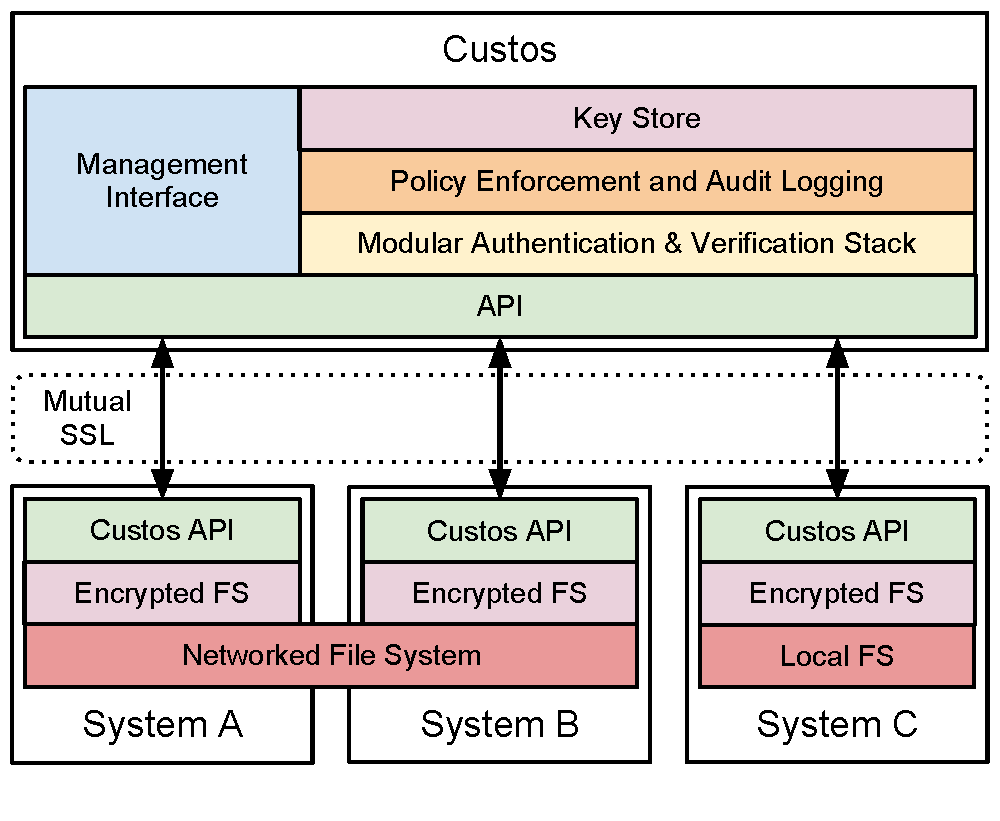
\includegraphics[width=\columnwidth]{./include/CustosOverview.pdf}
  \caption{Custos Architecture Overview}
  \label{fig:custosoverview}
\end{figure}

\subsection{Custos Key Request API}

The Custos Key Request API is the means by which encryption systems
access Custos. Through this API, Custos-integrated encryption systems
may perform operations like adding, deleting, accessing, or modifying
keys. We assume that Custos will primarily be used to store per-file
symmetric encryption keys, as symmetric keys and the encryption
methods associated with them provide the greatest degree of
flexibility for controlling file access on a per-file level. As such,
each key in Custos is mapped to the UUID of the file it was used to
encrypt. It is up to each encrypted file system to store the Custos
UUID for each file, but this is easily accomplished through the use of
file system provided extended attributes or separate databases. When a
system wishes to access or modify the key for a particular file in
Custos, it makes a call to the Custos API, providing the UUID for the
file in question as part of the request. In response, Custos will
establish a connection with the requesting system and request any
additional information required to authenticate the associated
actor. If the actor can be properly authenticated, and if Custos
determines that they are authorized to access the file, then Custos
will provide the key in question. Because the key exchange process
must be secure, we envision all Custos API interaction occurring over
a mutually-authenticated SSL connection or similar
bidirectionally-secured communication channel.

\subsection{Custos Authentication Modules}

\begin{figure}[!tb]
  \centering
  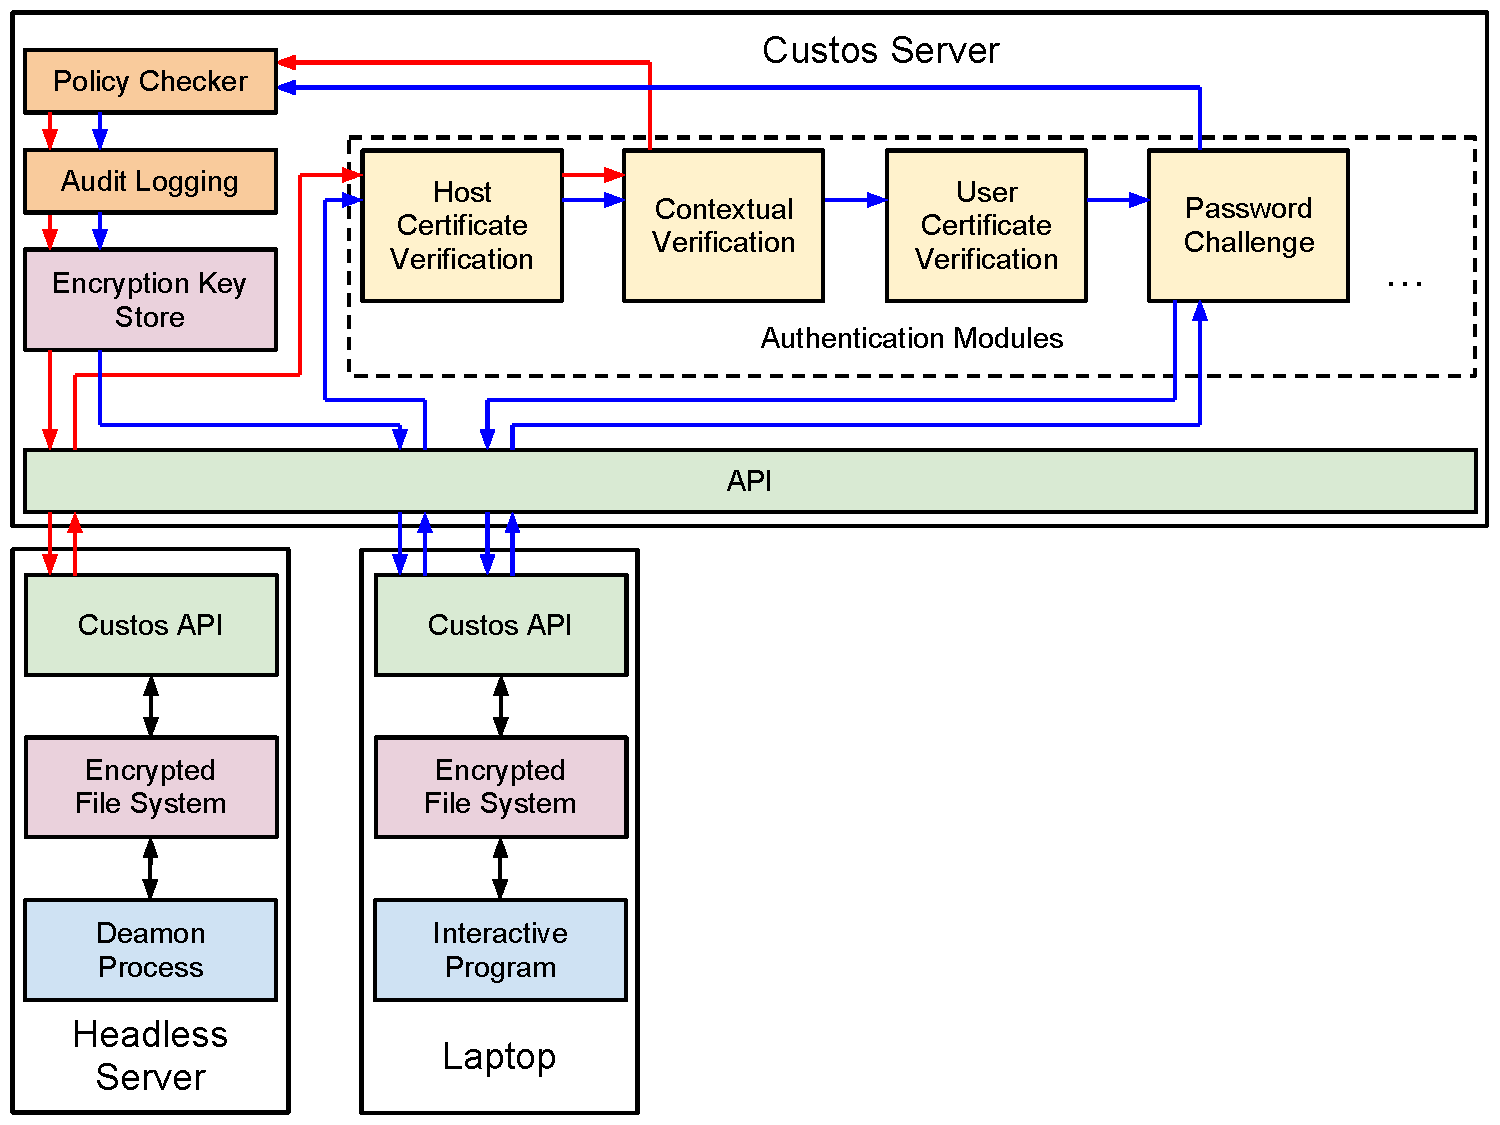
\includegraphics[width=\columnwidth]{./include/KeyRequest.pdf}
  \caption{Custos Key Request Examples}
  \label{fig:keyrequest}
\end{figure}

At Custos's core is its flexible support for a variety of
authentication and requirement modules. Custos provides a standardized
framework for adding modules. Each module verifies a specific
authentication or related requirement. Multiple modules can be chained
together in order to force Custos clients to meet multiple
requirements. Each key in Custos is associated with one or more module
chains, and access to that key will only be provided to clients that
can properly satisfy all modules in at least one valid chain. By
allowing multiple chains to be defined for each key, Custos enables
easy key sharing where different users can be required to supply
separate passwords, certificates, etc to access the same key. Custos
provides a handful of common modules by default, but also makes it
easy for users to add modules as needed via the extensible module
interface.

Since the Custos module system is at the heart of Custos's
flexibility, we envision using modules for a variety of authentication
methods. These include interactive authentication modules like simple
password-challenge modules that require the requesting actor to
provide a valid password or multi-factor-challenge modules that
require the user to posses a separate security device. They also
include non-interactive modules like public-private key modules to
authenticate specific actors or contextual security modules that place
limits on which network locations actors may access keys from, what
times of day keys can be accesses, or other environmental context
restraints \cite{Hulsebosch2005}. This range of modules, and the
ability to mix-and-match them to form separate authentication
requirements for each Custos key allows Custos to provide secure key
access in the widest possible variety of situations. For example,
Figure \ref{fig:keyrequest} shows two separate systems utilizing
Custos to access the required encryption keys to decrypt files on each
system. In the case of the Headless Server, only non-interactive
security modules are required for authentication, allowing a daemon
background process on the server to securely access an encrypted file
autonomously without requiring interactive human intervention. The
laptop, on the other hand, provides additional security by requiring
both interactive and non-interactive authentication methods,
appropriate for the protection of personal data that is only ever
accessed by a live user.

\subsection{Custos Management Interface}

Custos also provides a management interface via an additional API. We
envision such an API allowing for the easy construction of both web,
desktop, and command line based interfaces for managing Custos. The
management interface allows the Custos administrator to specify
authentication module chains for each key, to manually add, remove, or
modify keys, to revoke key access (as in the case of a stolen laptop,
etc), and to access the audit logs for a given key. This interface is
also where the settings for each module instance (shared secrets,
public keys, etc) are configured. Custos allows the user to define a
default authentication module chain that is automatically attached to
new keys as they are created. Per-file requirements that differ from
the default are then configured via the management interface. It is
important to note that this management interface is separate from the
Custos key access interface. We wish to encourage the separation of
authentication and access policy (controlled via the management
interface) from the underlying use of each key (via the key access
interface). This separation of policy and mechanism has proven
valuable in a variety of other systems, and we feel it serves Custos
well.
